%% Yuanhao Chen <yuanhao.chen.25@dartmouth.edu>
%% based on ACL 2023 template

\documentclass[11pt]{article}
\usepackage[hyperref, review]{acl}
\usepackage{font-settings}

\usepackage{enumitem}
\setlist[enumerate]{leftmargin=*, nosep, label={(\arabic*)}}

\usepackage{graphicx}
\graphicspath{{./images/}}
\usepackage{tabularray}
\UseTblrLibrary{booktabs}
\usepackage{caption}
\usepackage{float}
\usepackage{cleveref}
\crefname{figure}{Fig.\@}{Figs.\@}
\crefname{table}{Table}{Tables}

\usepackage{siunitx}

\usepackage{tikz}
\usetikzlibrary{shapes.geometric, arrows, positioning}
\tikzstyle{process} = [rectangle, draw, text centered, minimum height=2em]
\tikzstyle{io}=[trapezium, draw, text centered, trapezium left angle=60, trapezium right angle=120, minimum height=2em]
\tikzstyle{data}=[trapezium, rounded corners, draw, text centered, trapezium left angle=60, trapezium right angle=120, minimum height=2em]
\tikzstyle{connector} = [draw, -latex']

\title{\makebox[0pt]{Improving TTS for Shanghainese: Addressing Tone Sandhi via Word Segmentation}}
\def\outauthor{\begin{tabular}[t]{c}\bf Yuanhao Chen \\\texttt{yuanhao.chen.25@dartmouth.edu}\end{tabular}}
\date{}

\begin{document}

\maketitle

\begin{abstract}
    Tone is a crucial component of the prosody of Shanghainese, a Wu Chinese variety spoken primarily in urban Shanghai.
    Tone sandhi, which applies to all multi-syllabic words in Shanghainese, then, is key to natural-sounding speech. Unfortunately, recent work on Shanghainese TTS (text-to-speech) such as Apple's VoiceOver has shown poor performance with tone sandhi, especially LD (left-dominant sandhi).
    Here I show that word segmentation during text preprocessing can improve the quality of tone sandhi production in TTS models.
    Syllables within the same word are annotated with a special symbol, which serves as a prosodic annotation for the domain of LD.
    Contrary to the common practice of using prosodic annotation mainly for static pauses, this paper demonstrates that prosodic annotation can also be applied to dynamic tonal phenomena.
    I anticipate this project to be a starting point for bring formal linguistic accounts of Shanghainese into computational projects.
    Too long have we been using the Mandarin models to approximate Shanghainese, but it is a different language with its own linguistic features, and its digitisation and revitalisation should be treated as such.
\end{abstract}

\section{Introduction}
Shanghainese is a variety of Wu Chinese spoken primarily in urban Shanghai and globally by the Shanghainese diaspora.

Despite its formerly prominent status as a lingua franca in the Yangtze River Delta region, Shanghainese is now a minority language in Shanghai, with Putonghua (Standard Mandarin) being the dominant language in the city.
Furthermore, the situation is only exacerbated by the general sentiment among the younger generation that Shanghainese is a ``low-status'' language, and by their adoption of the linguistic model that one nation should use only one language \citep{gillilandLanguageAttitudesIdeologies2006}.
Education plays a crucial role in this process, as this sentiment was mainly observed among college students.
As a result, most young people in Shanghai, whether native or an immigrant, are unable to speak Shanghainese fluently \citep{wengSecondGenerationNew2023}.

With Putonghua being the perceived authentic and superior language in many aspects of life, crucially including education, it is direly important to preserve the linguistic variety in Shanghai by promoting the use of Shanghainese.
Digitisation of a substratum is an effective way to promote the language in teaching, learning, and various other dimensions of cultural life \citep{villaIntegratingTechnologyMinority2002}.

In this project, I aim to build a TTS (text-to-speech) system for Shanghainese, which is a crucial component in the digitisation of a language, serving as a bridge between the digitised written spoken forms of the language.
This is not to say that there is no existing work on Shanghainese TTS. Notably, \citet{VoiceOver} added Shanghainese to the list of languages supported by VoiceOver, the screen reader built into Apple's operating systems. However, the quality of the synthesised speech is not satisfactory, and definitely not on par with the quality of the synthesised speech for other Sinitic languages such as Putonghua.
The main problem with Shanghainese Voice\-Over is its occasional poor performance with tone sandhi, especially LD (left-dominant sandhi), a suprasegmental phonological process involving a specific bounding domain \citep{robertsAutosegmentalMetricalModelShanghainese2020}.
For example, the word /[zɑ̃²³.he³³⁴]\textsubscript{LD domain}/ `Shanghai' has to be pronounced with LD as [zɑ̃².he⁴] (the left syllable's rising contour is spread over to the right one).

This paper will explore the possibility of improving tone sandhi in Shanghainese TTS by putting focus on annotating the bounding domain of LD during preprocessing of input texts.
Specifically, I will segment the input text into lexical words. My results confirm that this approach is effective in improving the quality of synthesised speech in terms of tone sandhi.

\section{Methodology}
\subsection{Overview}
The key to improving LD in Shanghainese TTS is to annotate the bounding domain of LD.
Instead of training a model for this task, which is difficult due to lack of resources, I will perform word segmentation, because lexical words highly correlates with the domains for LD \citep{kuangToneRepresentationTone2019}; formally, LD domains can be formed by the left edges of lexical words, with a few exceptions \citep{robertsAutosegmentalMetricalModelShanghainese2020}.
Thus, this prosodic annotation can be transformed into word segmentation, giving us the overall pipeline of this paper as shown in \cref{fig:pipeline}.
\begin{figure*}
    \centering
    \makebox[0pt]{
        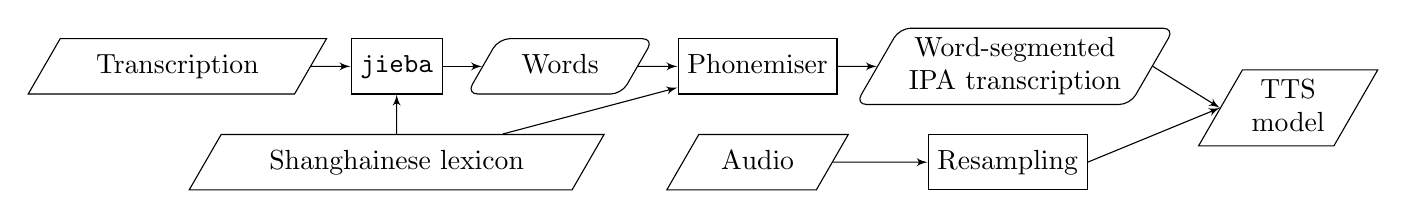
\begin{tikzpicture}[node distance=0.5cm, align=center, style={font=\vphantom{Ag}}]
            \node[io] (transcription) {Transcription};
            \node[process, right=of transcription] (jieba) {\texttt{jieba}};
            \node[io, below=of jieba] (sh_lex) {Shanghainese lexicon};
            \node[data, right=of jieba] (seg_words) {Words};
            \node[process, right=of seg_words] (phon) {Phonemiser};
            \node[data, right=of phon] (seg_ipa) {Word-segmented\\IPA transcription};

            \node[io, below=of phon] (audio) {Audio};
            \node[process, right=of audio, xshift=2em] (downsample) {Resampling};

            \node[io, right=of seg_ipa, yshift=-1.5em, xshift=1em] (tts) {TTS\\model};

            \draw[connector] (transcription) -- (jieba);
            \draw[connector] (jieba) -- (seg_words);
            \draw[connector] (sh_lex) -- (jieba);
            \draw[connector] (seg_words) -- (phon);
            \draw[connector] (phon) -- (seg_ipa);
            \draw[connector] (seg_ipa.east) -- (tts.west);
            \draw[connector] (sh_lex) -- (phon);

            \draw[connector] (audio) -- (downsample);
            \draw[connector] (downsample.east) -- (tts.west);
        \end{tikzpicture}
    }
    \caption{Overview of the pipeline in training the TTS model, with emphasis on the text preprocessing steps.\label{fig:pipeline}}
\end{figure*}

\subsection{Datasets}
% shh.dict.cn 5607 seconds, 2012 files
The data basis of TTS models is a list of corresponding audio files and transcriptions.
I am using a dataset of an ASR project \citep{cosmos-breakCosmosBreakAsr2023}, which contains 2,012 audio files and corresponding transcriptions in Chinese characters, totalling 5,607 seconds of speech of a single Shanghainese speaker. The types of speech in the dataset range from single words to phrases and sentences.
The audio is resampled to 16kHz for training.

For word segmentation and phonemisation, we are going to need a phonemically annotated lexicon of Shanghainese. I am using one containing more than 125,000 lexical entries, 51,000 of which have corresponding romanisations \citep{yuanhaochenRimeYahweZaonhe2022}.

\subsection{Word Segmentation}
The \texttt{jieba} library is the most popular open-source Chinese word segmentation library, which comes with a Mandarin dictionary out of the box \citep{junyiJieba2023}.
It implements two models, namely a trie of a deterministic finite automaton (DFA) pre-built from the dictionary, and a hidden Markov model (HMM) with Viterbi algorithm as a backup for unknown words.
% We will have to rely on the Mandarin dictionary as our basis as the Shanghainese dictionary contains no frequency information, but we will add high frequencies to Shanghainese lexicon. This should work well as written Mandarin and Shanghainese are very similar.
We will have to rely on the Mandarin dictionary because word-segmentation algorithms require word frequency information, which is not available in the Shanghainese lexicon, but we can patch the model by adding weights to Shanghainese-specific words on top of Mandarin weights. This works well, as written Mandarin and Shanghainese are very similar.

\subsection{Phonemisation}
The aforementioned dictionary \citep{yuanhaochenRimeYahweZaonhe2022} is used to romanise segmented words in \emph{Yahwe} Wu Chinese Romanisation (吳語協會式拼音).
As the dictionary only contains traditional forms, before romanising, the words are converted to Traditional Chinese using \citet{kuoOpenChineseConvert2023}.
Then, \texttt{Qieyun} \citep{Qieyunpython2022} is used to add any necessary tone numbers to the romanisation.
The romanisation is then converted to broad IPA transcription largely following the paradigm of \citet{qianShanghaiFangYan2007}. Because the goal is not to accurately transcribe phonetically but to effectively feed the TTS model with phonemic contrasts, some notational techniques are employed to reduce the number of ambiguous digraphs, such as using ⟨c⟩ for /tɕ/ and ⟨ɟ⟩ for /dʑ/.

\subsection{Training the TTS Model}
The TTS model presented in this paper is trained using the VITS end-to-end TTS model \citep{kimConditionalVariationalAutoencoder2021}.
Compared to previous popular TTS models such as Glow-TTS \citep{kimGlowTTSGenerativeFlow2020}, VITS employs a variational autoencoder (VAE) to produce a latent model of the input text and a stochastic duration predictor, which allows the model to  express the natural one-to-many relationship in which a text input can be spoken in multiple ways with different pitches and rhythms.

This is perfect for the task that this paper aims to accomplish: The model can effectively learn that the same string in the input may be pronounced with a different pitch depending on whether tone sandhi applies, i.e., depending on the prosodic environment.

The pre-processed text and audio are fed into the VITS model, which is trained for 50K steps with a batch size of 32.

\section{Experiments}
I conducted an $n \times 3 \times 5 \times 4$ experiment, where $n=11$ is the number of native Shanghainese participants, 3 is the number of speakers generating the audio samples, 5 is the number of sentences, and 4 is the number of metrics. A subjective human evaluation (MOS, mean opinion score) is conducted under each condition on a 1--5 scale, with 5 being the best (see details in \cref{fig:questionnaire}).

The three speakers are
\begin{enumerate}
    \item The model presented by this paper.
    \item Shanghainese VoiceOver \citep{VoiceOver}.
    \item This paper's author, a native speaker.
\end{enumerate}

% The five sentences are
% \begin{enumerate}
%     \item 我老衰瘏個,昨日夜里睏弗着。 `It is so agonising that I couldn't fall asleep last night,' a sentence slightly modified from the training data.
%     \item 上海是一座國際化大都市。 `Shanghai is an international metropolis,' a sentence randomly generated by ChatGPT.
%     \item 虹橋機場分爲一號航站樓搭兩號航站樓。 `Hongqiao Airport is divided into Terminal 1 and Terminal 2,' a sentence taken from \href{https://wuu.wikipedia.org/wiki/%E4%B8%8A%E6%B5%B7%E8%99%B9%E6%A9%8B%E5%9C%8B%E9%9A%9B%E6%A9%9F%E5%A0%B4}{the Wikipedia article on Hongqiao Airport}.
%     \item 儂好,世界! `Hello, world!' a common phrase in programming.
%     \item 儂弗要弗二弗三個。 `Don't be nasty,' a common Shanghainese saying.
% \end{enumerate}

% 1. Comprehensibility: How well can you understand the meaning of the audio?
% 2. Naturalness: How natural does the audio sound?
% 3. Accuracy: How well does the audio match how a native speaker like you would pronounce it?
% 4. Intelligibility: How much effort does it take to make sense of the audio?
The four metrics are as proposed by \citet{cardosoEvaluatingTexttospeechSynthesizers2015}:
\begin{enumerate}
    \item Comprehensibility: How well can you understand the meaning of the audio?
    \item Naturalness: How natural does the audio sound?
    \item Accuracy: How well does the audio match how a native speaker like you would pronounce it?
    \item Intelligibility: How much effort does it take to make sense of the audio?
\end{enumerate}

\section{Results}
\subsection{Tone Sandhi production}
In all test sentences (containing 23 different LD domains to trigger sandhi), all speakers produce the correct tone sandhi, except for VoiceOver, which fails to produce the correct tone sandhi in sentence 5, 儂弗要弗二弗三個 `don't be nasty'.

弗二弗三個 `nasty' /[vəʔ¹².ɲi²³.vəʔ¹².se⁵¹.ɦəʔ]\textsubscript{LD}/ is a word forming a pentasyllabic LD domain, which should surface tonally as [vəʔ¹.ɲi³.vəʔ².se².ɦəʔ¹], but VoiceOver incorrectly treats it as /[vəʔ¹².ɲi²³]\textsubscript{LD} [[vəʔ¹².se⁵¹.ɦəʔ]\textsubscript{LD} \ldots]\textsubscript{RD}/, splitting the word into two LD domains, and assuming that an extra RD (right-dominant sandhi) domain dominates the second LD domain, which is doubly wrong. This produces the incorrect surface form [vəʔ¹.ɲi³ vəʔ¹.se¹.ɦəʔ³].
Compare the pitch in \cref{fig:s5_sp2,fig:s5_sp3}.

\subsection{Questionnaire}
One out of 11 questionnaires collected is discarded for being incomplete. The valid $10 \times 3 \times 5 \times 4$ opinion scores are used for various statistical analyses.

The overall MOS of three speakers are shown in \cref{tab:overall_mos}. Speakers 1 and 2 are not significantly different from each other ($p=0.64$); they both have significantly lower scores than speaker 3 ($p\ll 0.001$).
A breakdown of scores grouped by metrics shows similar statistical relationships between speakers (see \cref{tab:mos_by_metrics}).

In a breakdown of scores grouped by sentences, two statistically significant differences are found: Speaker 1 has a significantly lower score than speaker 2 in sentence 2, and speaker 2 has a significantly lower score than speaker 1 in sentence 5 (both $p\ll 0.001$; see \cref{tab:mos_by_sentences}).

\section{Discussion}
From the comparison of overall MOS and the comparison of MOS grouped by metrics, we can see that the human acceptability of this model is generally comparable to that of VoiceOver.
Statistically significant differences emerge when we break down the scores by sentences, showing that both models have their own strengths and weaknesses.

\subsection{Shortcomings of this model}
As shown in \cref{tab:mos_by_sentences}, this model has a significantly lower score than VoiceOver in sentence 2, 上海是一座國際化大都市 `Shanghai is an international metropolis'.

There are tonal differences between what this model (\cref{fig:s2_sp1}) produces for 國際化大都市 `international metropolis' /koʔ⁵.tɕi⁵³.ho³³⁴ da²³.tu⁵³.zz̩²³/ and what VoiceOver (\cref{fig:s2_sp2}) and I (\cref{fig:s2_sp3}) produce.
However, this is not the reason for the low score, because this phrase indeed has two alternative prosodic segmentation possibilities: /[[koʔ⁵.tɕi⁵³.ho³³⁴]\textsubscript{LD} [da²³.tu⁵³.zz̩²³]\textsubscript{LD}]\textsubscript{RD}/ (what this model goes for) and /[[koʔ⁵.tɕi⁵³.ho³³⁴]\textsubscript{LD}]\textsubscript{RD} [[da²³.tu⁵³.zz̩²³]\textsubscript{LD}]\textsubscript{RD}/ (what the other speakers go for), depending on whether `international' and `metropolis' are grouped together in an RD domain.

The main issue with the pronunciation of this model is that the syllable /koʔ/ is produced too long compared to syllables without /-ʔ/ coda. In Shanghainese, the glottal stop coda is often realised as the shortening of the nucleus (giving [kŏ]), instead of actually pronounced.
However, this model produces a syllable clearly longer than others, with a duration of \qty{0.28}{s}, or $10\%$ of total speech duration, whereas the native speaker produces this with a duration of \qty{0.16}{s}, or $6\%$ of total speech duration.

This behaviour is possibly due to VITS's makeshift treatment of blanks in speech --- VITS inserts a \texttt{BLANK} token between every input character, which supposedly enhances performance in general \citep{kimConditionalVariationalAutoencoder2021}. $25\%$ of the duration of /koʔ/ is actually nearly silence at the end of the syllable, a weird pause to have within a word.
% mitigating: Zhang et al.: use more prosodic annotations PW, PP, IP

\subsection{Advantages of this model}
The model presented by this paper is significantly better than VoiceOver in sentence 5, because it correctly handles LD of /[vəʔ¹².ɲi²³.vəʔ¹².se⁵¹.ɦəʔ]\textsubscript{LD}/, which VoiceOver fails (compare \cref{fig:s5_sp1,fig:s5_sp2} to the native speaker version in \cref{fig:s5_sp3}).

This difference is manifested by the mostly correct word segmentation of this model, which outputs \texttt{vəʔ-ɲi=vəʔ=se1 gəʔ}, where hyphens connect syllables in a known word and double hyphens connect those in an inferred word; \texttt{gəʔ} (/ɦəʔ/ when cliticised) is left out but can be inferred from context by the TTS model because it is a common suffix that clings to the previous word.
Admittedly, this result might be improved even further if we train a dedicated prosodic annotation model that can detect clitics, rather than just word-segmentation, but the current result is already satisfactory.

The output of VoiceOver is also correct under a low-high pitch accent analysis of Shanghainese \citep{robertsAutosegmentalMetricalModelShanghainese2020}, which predicts a pitch contour of LHLLL for this word. However, to sound more tonally natural, one has to correctly formulate LD domains to get the exact pitch contour, which further highlights the importance of accurate prosodic structure in Shanghainese.

\subsection{Ethical considerations of this project}
The nature of TTS models is to mimic human speech as perfectly as possible.
With progress in more natural-sounding TTS models such as the one in this paper, it is possible to use TTS models to impersonate other people's voices, which can be used for malicious purposes such as fraud.
More concerningly, voice conversion is easy to do with TTS models with VAE such as VITS, which drastically widens the potential scope of malicious use to any person.
While driving the digitisation and revitalisation of a minority language like Shanghainese, we should simultaneously be aware of the potential harm that technology can bring, and definitely refrain from any malicious application.

\section{Conclusion}
In this work, I have presented a TTS model for Shanghainese with the novel approach of emphasising bounding domains of tone sandhi, specifically LD, during text preprocessing. Due to lack of material to train a dedicated annotation model, word segmentation is employed as a proxy for this phonological information, which is shown to be effective in improving the tone sandhi quality of the output speech compared to \citet{VoiceOver}. Further improvement in performance of timing and pausing may be achieved by switching to a TTS model that handles blanks in speech better.

Beyond just prosody, the significance of this project should be to raise awareness of the importance of a formal linguistic account in every aspect of the development of computational systems regarding Shanghainese.
For example, in the dataset used in this project is originally for an ASR project \citep{cosmos-breakCosmosBreakAsr2023}, but the transcription is scattered with 假借 (phonetic loan characters), where a character is used for its Mandarin pronunciation to approximate the ``dialectic'' pronunciation, likely because the transcriber read fluently only in Mandarin. For example, 萨 (a surname, Mandarin /sa/) is used for 啥 (`what', Shanghainese /sa/); such practice is common but greatly hinders a consistent and formal treatment of Shanghainese orthography and lexicon in computational systems, as the character used to approximate varies from person to person, and the phenomenon itself is a manifestation of Mandarin centralism which marginalises Shanghainese.

Specific to the topic of this project, the lack of a computational model implemented as per a formal linguistic account of Shanghainese tone system is a major obstacle to the improvement of tonal performance in TTS. Even word segmentation, which is a makeshift solution of prosodic annotation, is carried out by the makeshift approach of using the Mandarin--pre-trained \texttt{jieba} model.

In general, despite the low-resource status of most substrata, it is important to be alerted that over-reliance on resources of the superstratum is only a makshift solution that can both undermine the authenticity of the result and take the focus away from the development of the scaffolding (implementation of formal linguistic accounts) of substrata.
Therefore, to engineer reliable and minority-friendly computational systems, further research should really put the development of the scaffolding of substrata at the top of the agenda.

% bib
\bibliography{main}
\bibliographystyle{acl_natbib}

\onecolumn
\appendix
\section{Tables}
\begin{table}[H]
    \centering
    \begin{tblr}{
            columns = {c},
            cell{2-Z}{2-Z} = {mode=math, font={\figureversion{tabular}}},
        }
        \toprule
        Speaker & Overall MOS   \\
        \midrule
        1       & 4.14 \pm 0.12 \\
        2       & 4.19 \pm 0.14 \\
        3       & 4.83 \pm 0.06 \\
        \bottomrule
    \end{tblr}
    \caption{Overall MOS of three speakers. Confidence interval: $95\%$; same for tables below.\label{tab:overall_mos}}
\end{table}

\begin{table}[H]
    \centering
    \begin{tblr}{
            columns = {c},
            cell{2-Z}{2-Z} = {mode=math, font={\figureversion{tabular}}},
        }
        \toprule
        Speaker & Accuracy      & Comprehensibility & Intelligibility & Naturalness   \\
        \midrule
        1       & 4.06 \pm 0.26 & 4.48 \pm 0.17     & 4.36 \pm 0.22   & 3.66 \pm 0.28 \\
        2       & 4.02 \pm 0.36 & 4.58 \pm 0.18     & 4.38 \pm 0.24   & 3.76 \pm 0.32 \\
        3       & 4.82 \pm 0.11 & 4.82 \pm 0.11     & 4.86 \pm 0.10   & 4.82 \pm 0.14 \\
        \bottomrule
    \end{tblr}
    \caption{MOS of three speakers by metrics.\label{tab:mos_by_metrics}}
\end{table}

\begin{table}[H]
    \centering
    \begin{tblr}{
            columns = {c},
            cell{2-Z}{2-Z} = {mode=math, font={\figureversion{tabular}}},
        }
        \toprule
        Speaker & Sentence 1    & Sentence 2    & Sentence 3    & Sentence 4    & Sentence 5    \\
        \midrule
        1       & 4.35 \pm 0.22 & 3.70 \pm 0.34 & 3.85 \pm 0.28 & 4.28 \pm 0.25 & 4.53 \pm 0.24 \\
        2       & 4.45 \pm 0.24 & 4.70 \pm 0.18 & 4.15 \pm 0.26 & 4.55 \pm 0.24 & 3.08 \pm 0.41 \\
        3       & 4.83 \pm 0.12 & 4.82 \pm 0.12 & 4.88 \pm 0.13 & 4.75 \pm 0.16 & 4.88 \pm 0.11 \\
        \bottomrule
    \end{tblr}
    \caption{MOS of three speakers by sentences.\label{tab:mos_by_sentences}}
\end{table}

\section{Figures}
\begin{figure}[H]
    \centering
    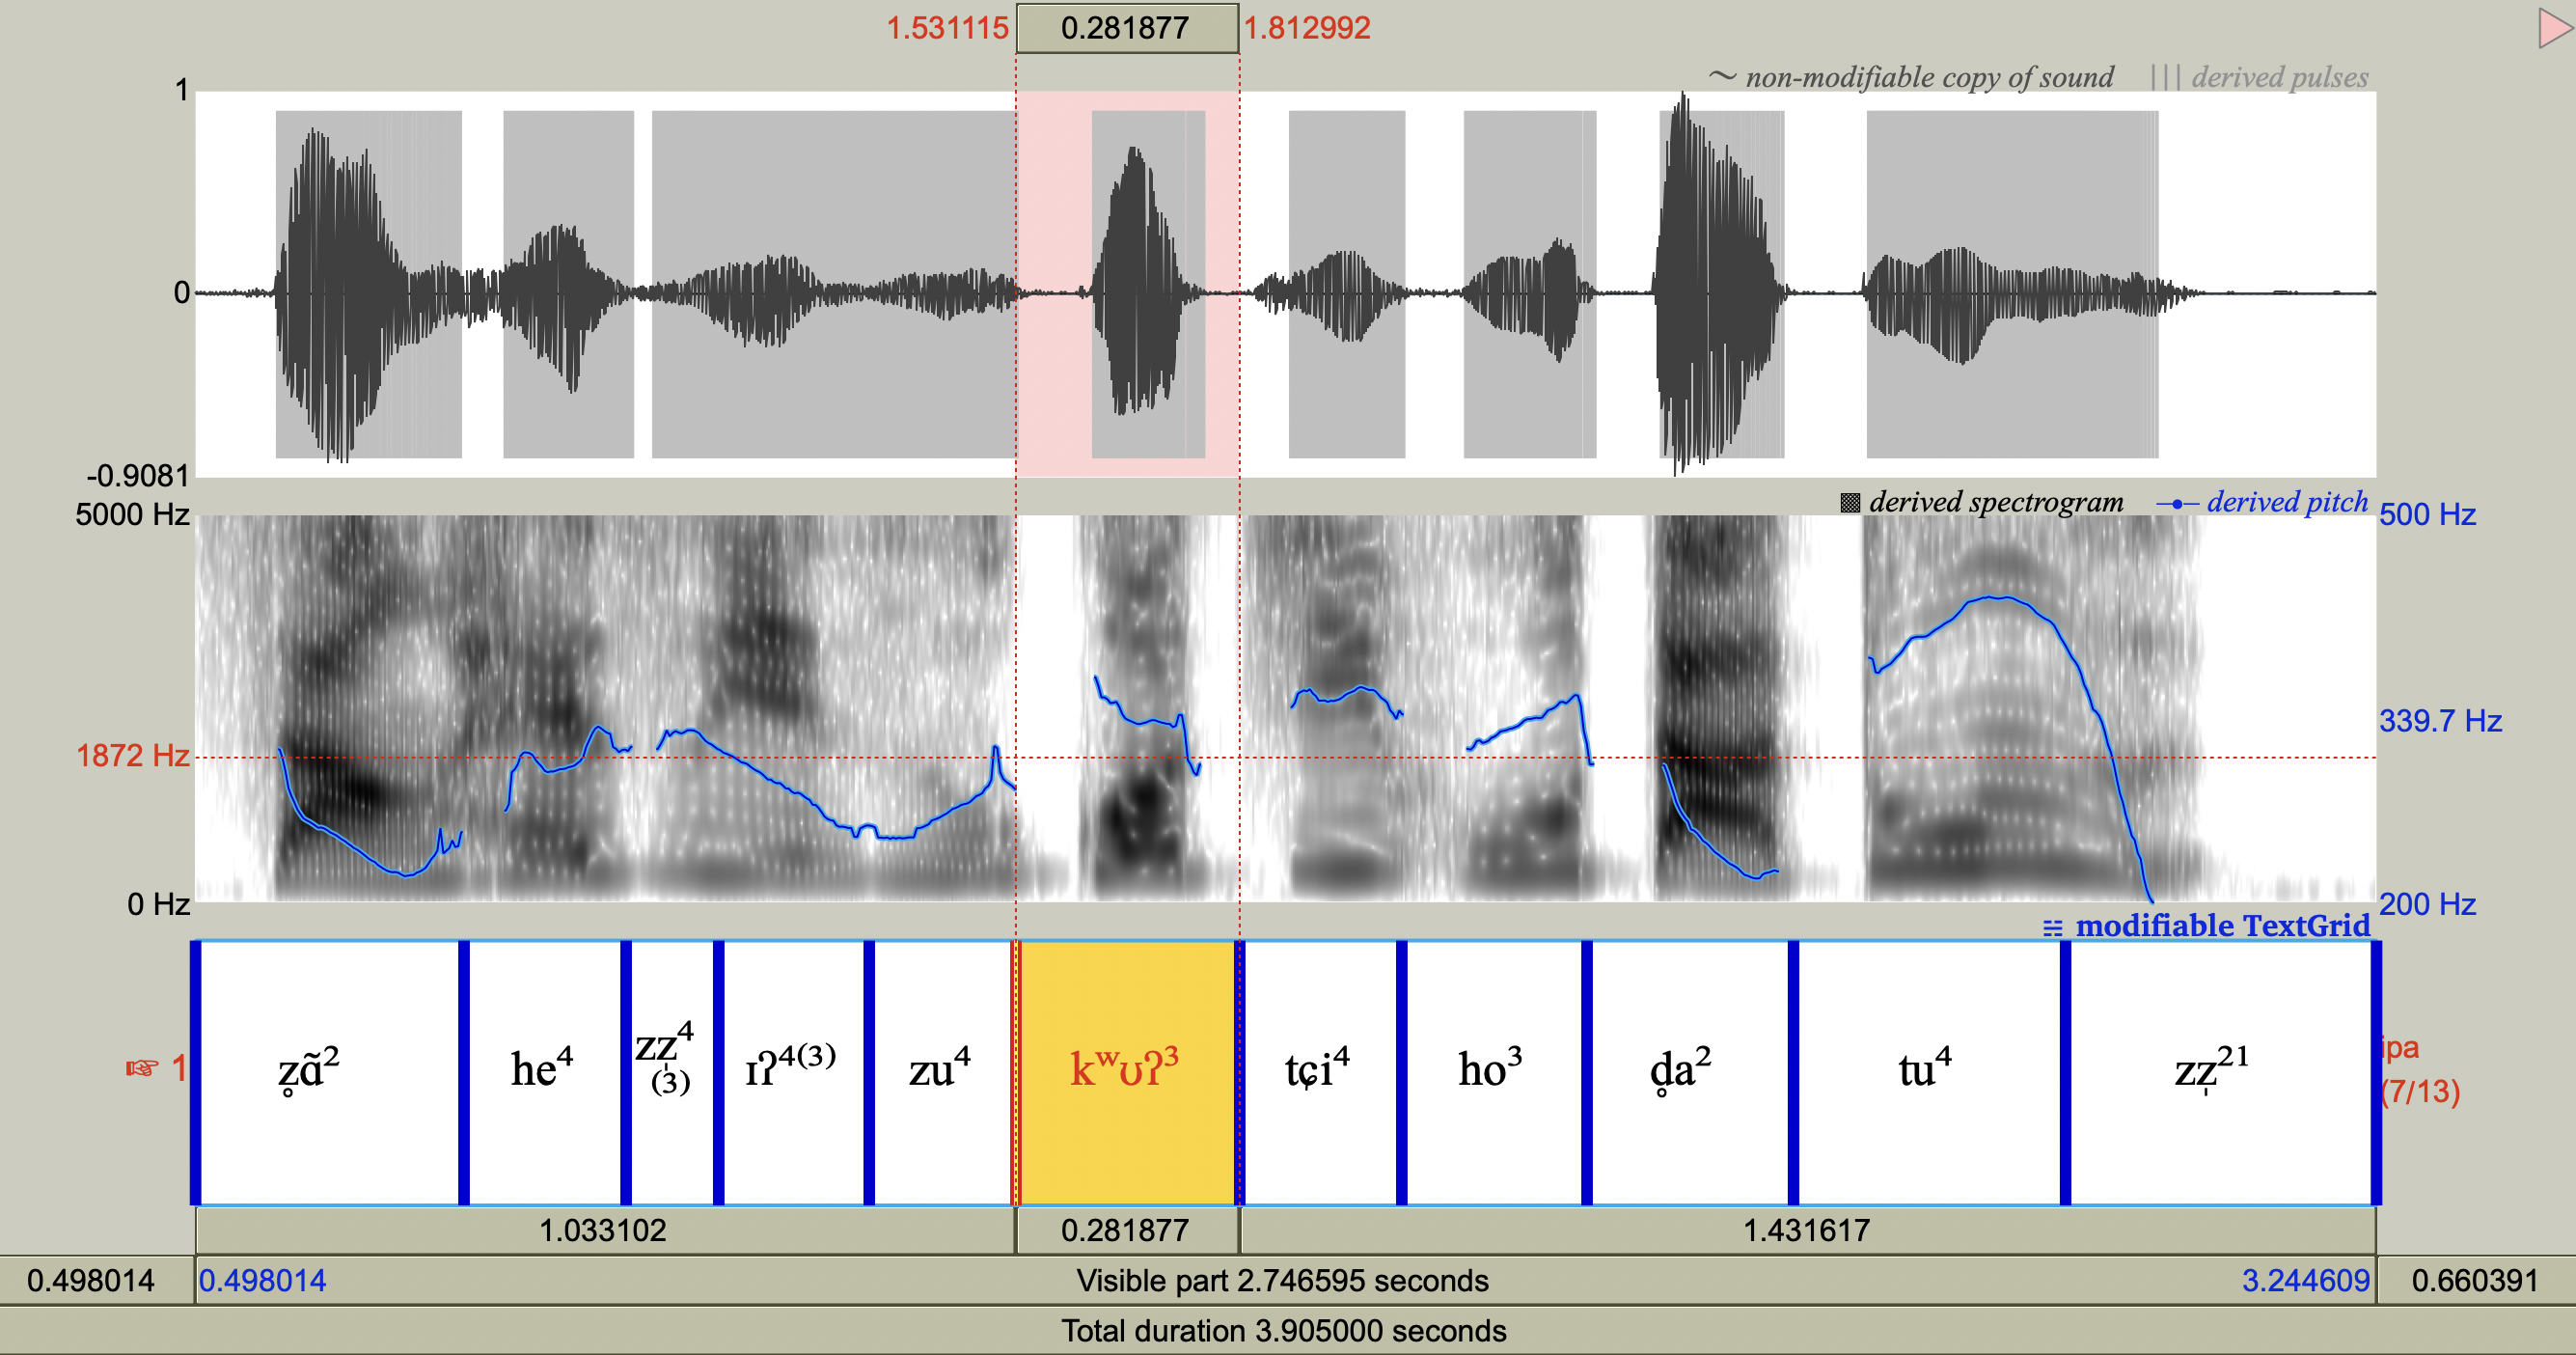
\includegraphics[width=0.6\paperwidth]{s2_sp1.png}
    \caption{Sentence 2 by speaker 1 with broad phonetic annotation. Tones are represented by Chao tone letters as their phonetic realisations. Parentheses indicate uncertain tone height that is within acceptable range and not crucial to the analysis. Same for figures below.\label{fig:s2_sp1}}
\end{figure}

\begin{figure}[H]
    \centering
    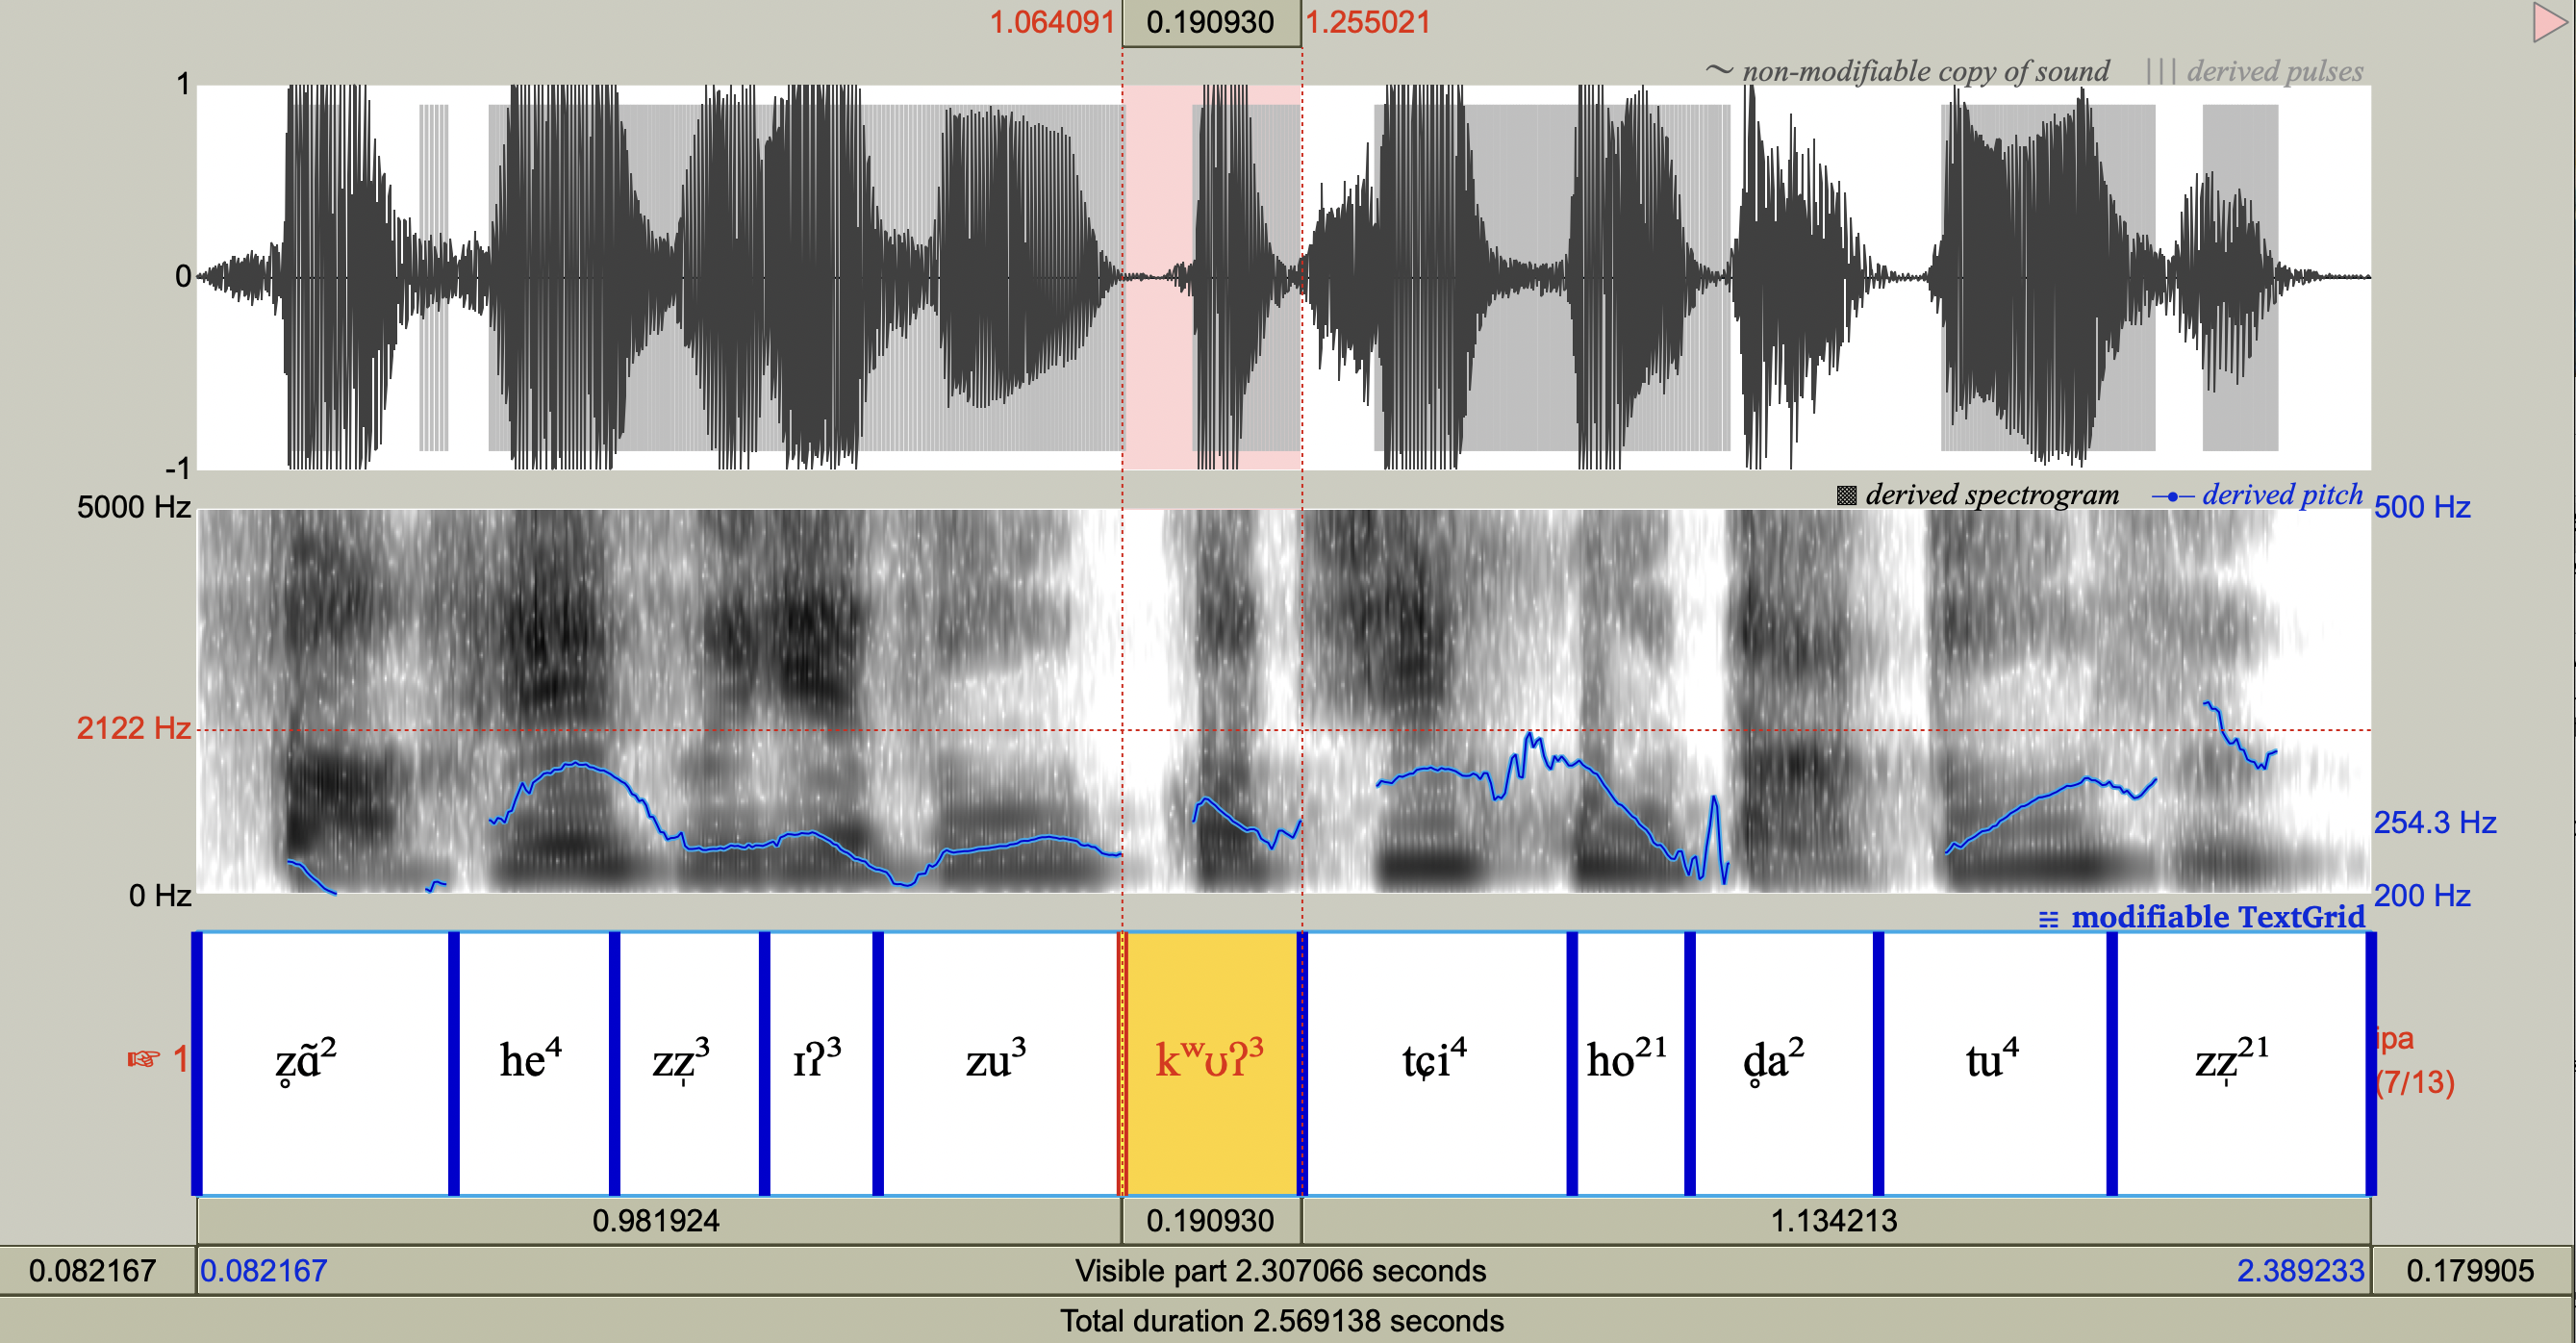
\includegraphics[width=0.6\paperwidth]{s2_sp2.png}
    \caption{Sentence 2 by speaker 2.\label{fig:s2_sp2}}
\end{figure}

\begin{figure}[H]
    \centering
    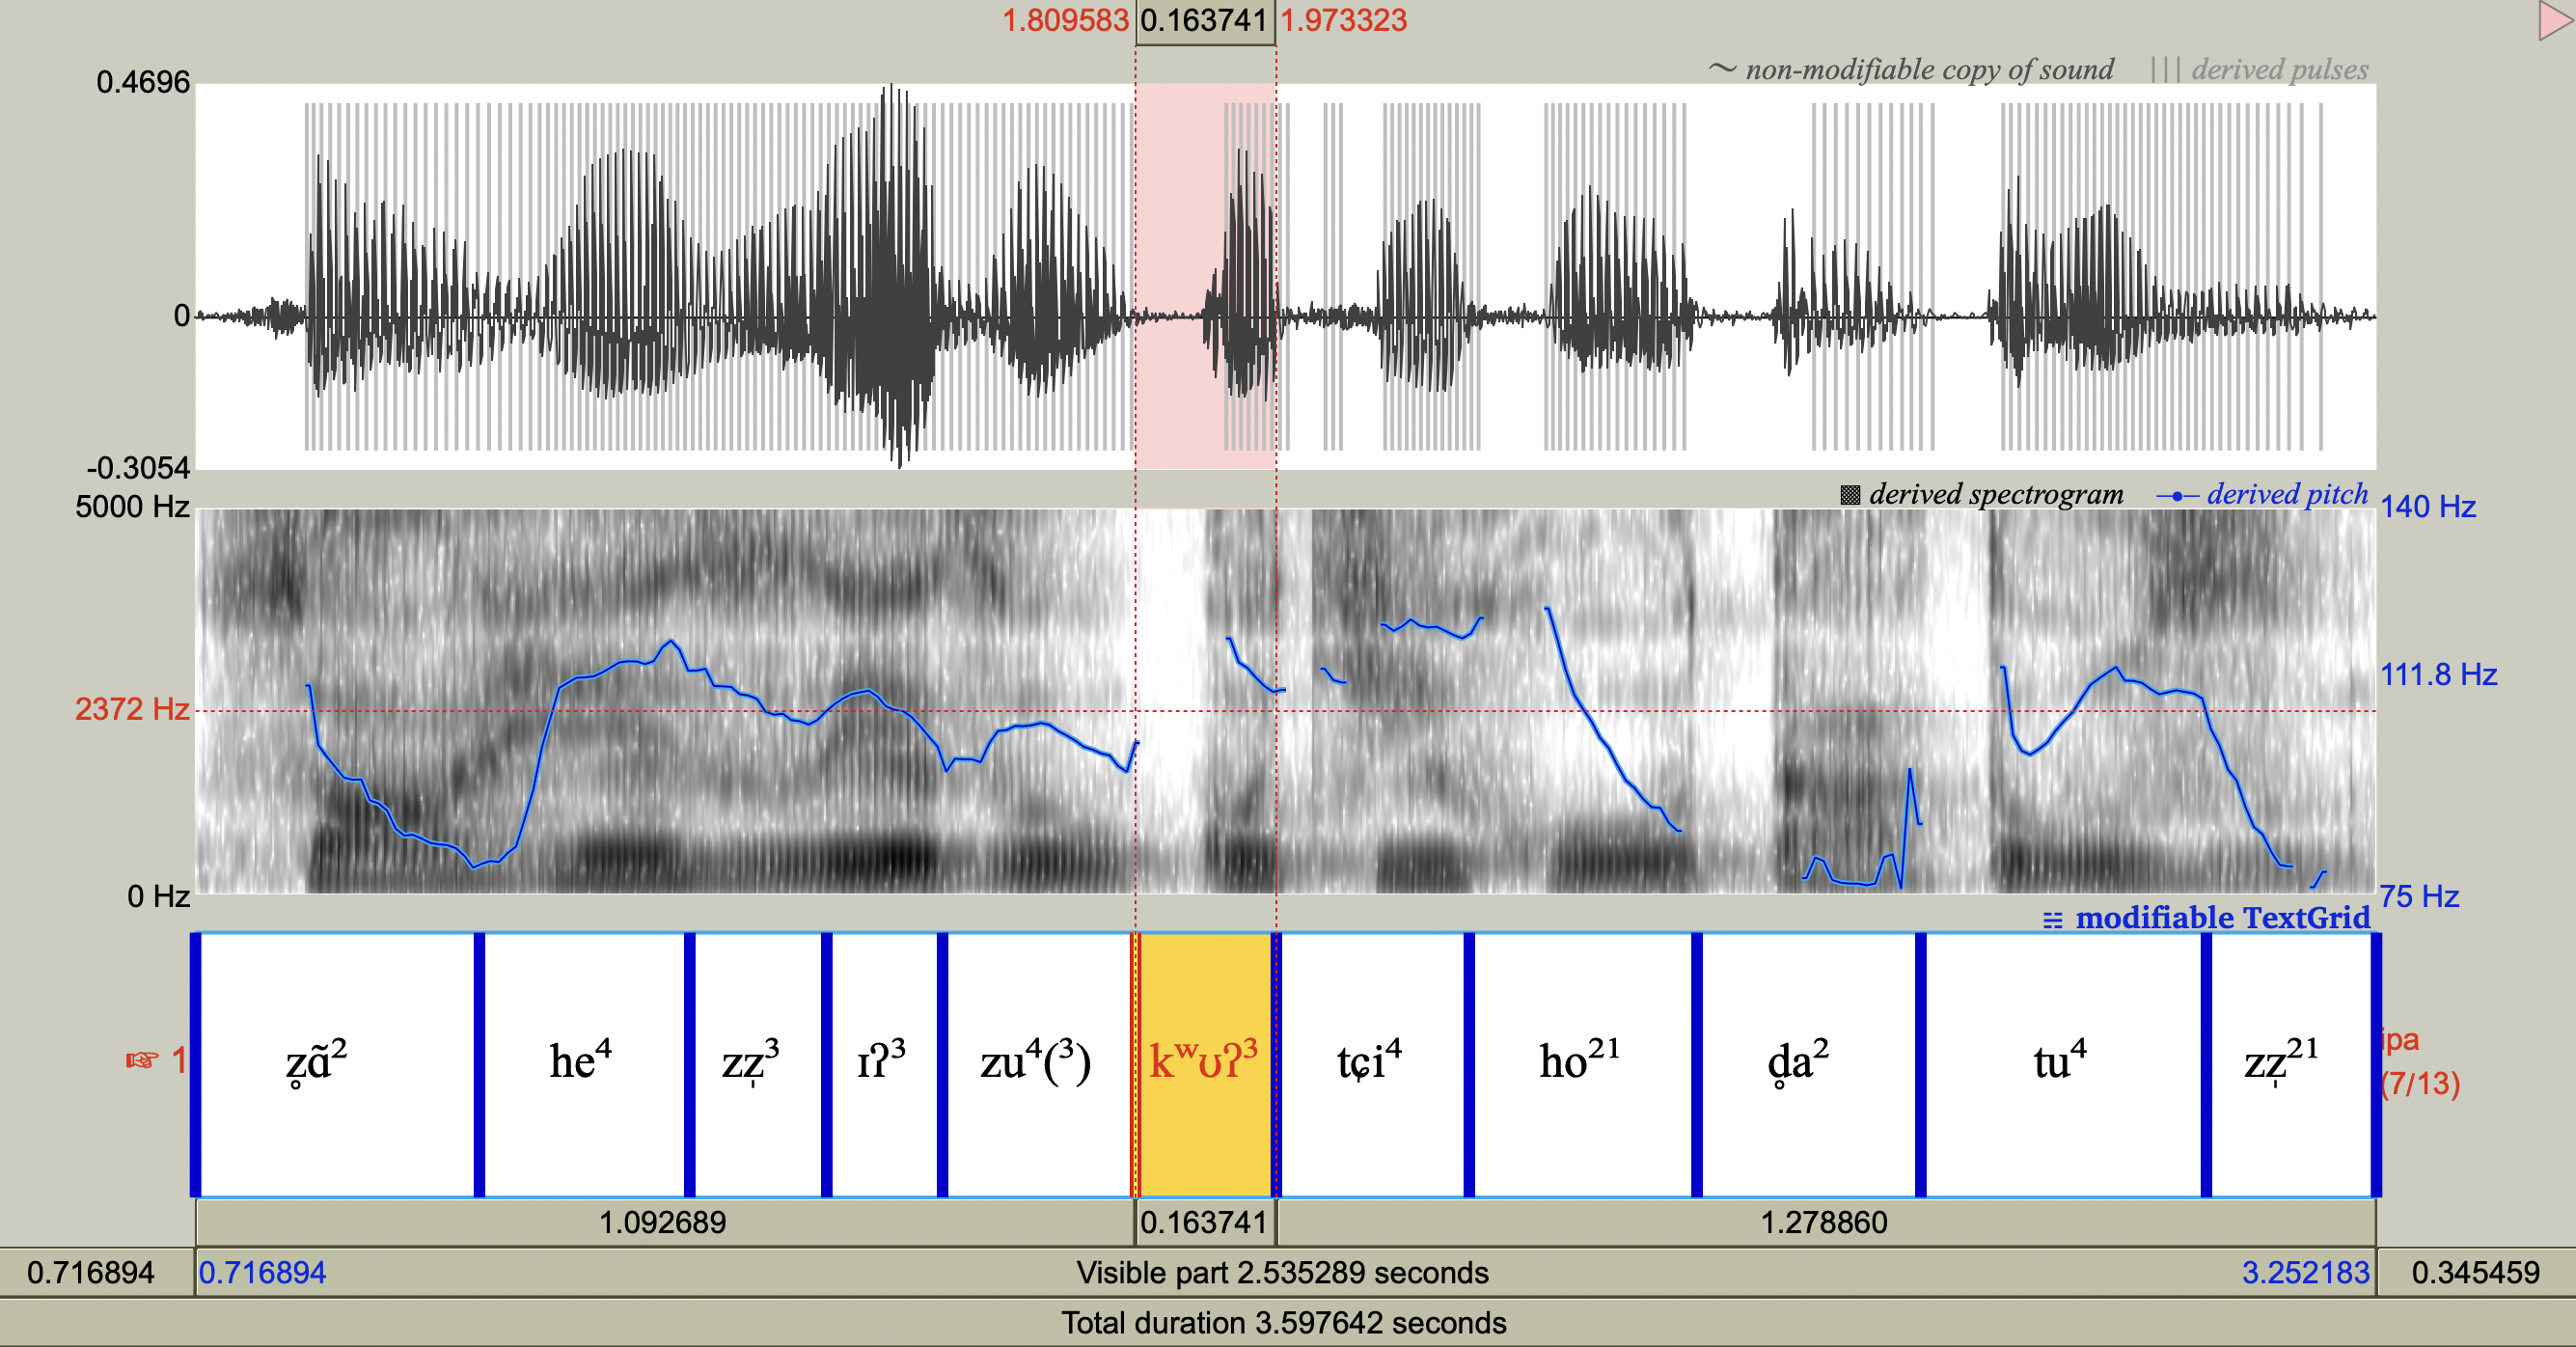
\includegraphics[width=0.6\paperwidth]{s2_sp3.png}
    \caption{Sentence 2 by speaker 3.\label{fig:s2_sp3}}
\end{figure}

\begin{figure}[H]
    \centering
    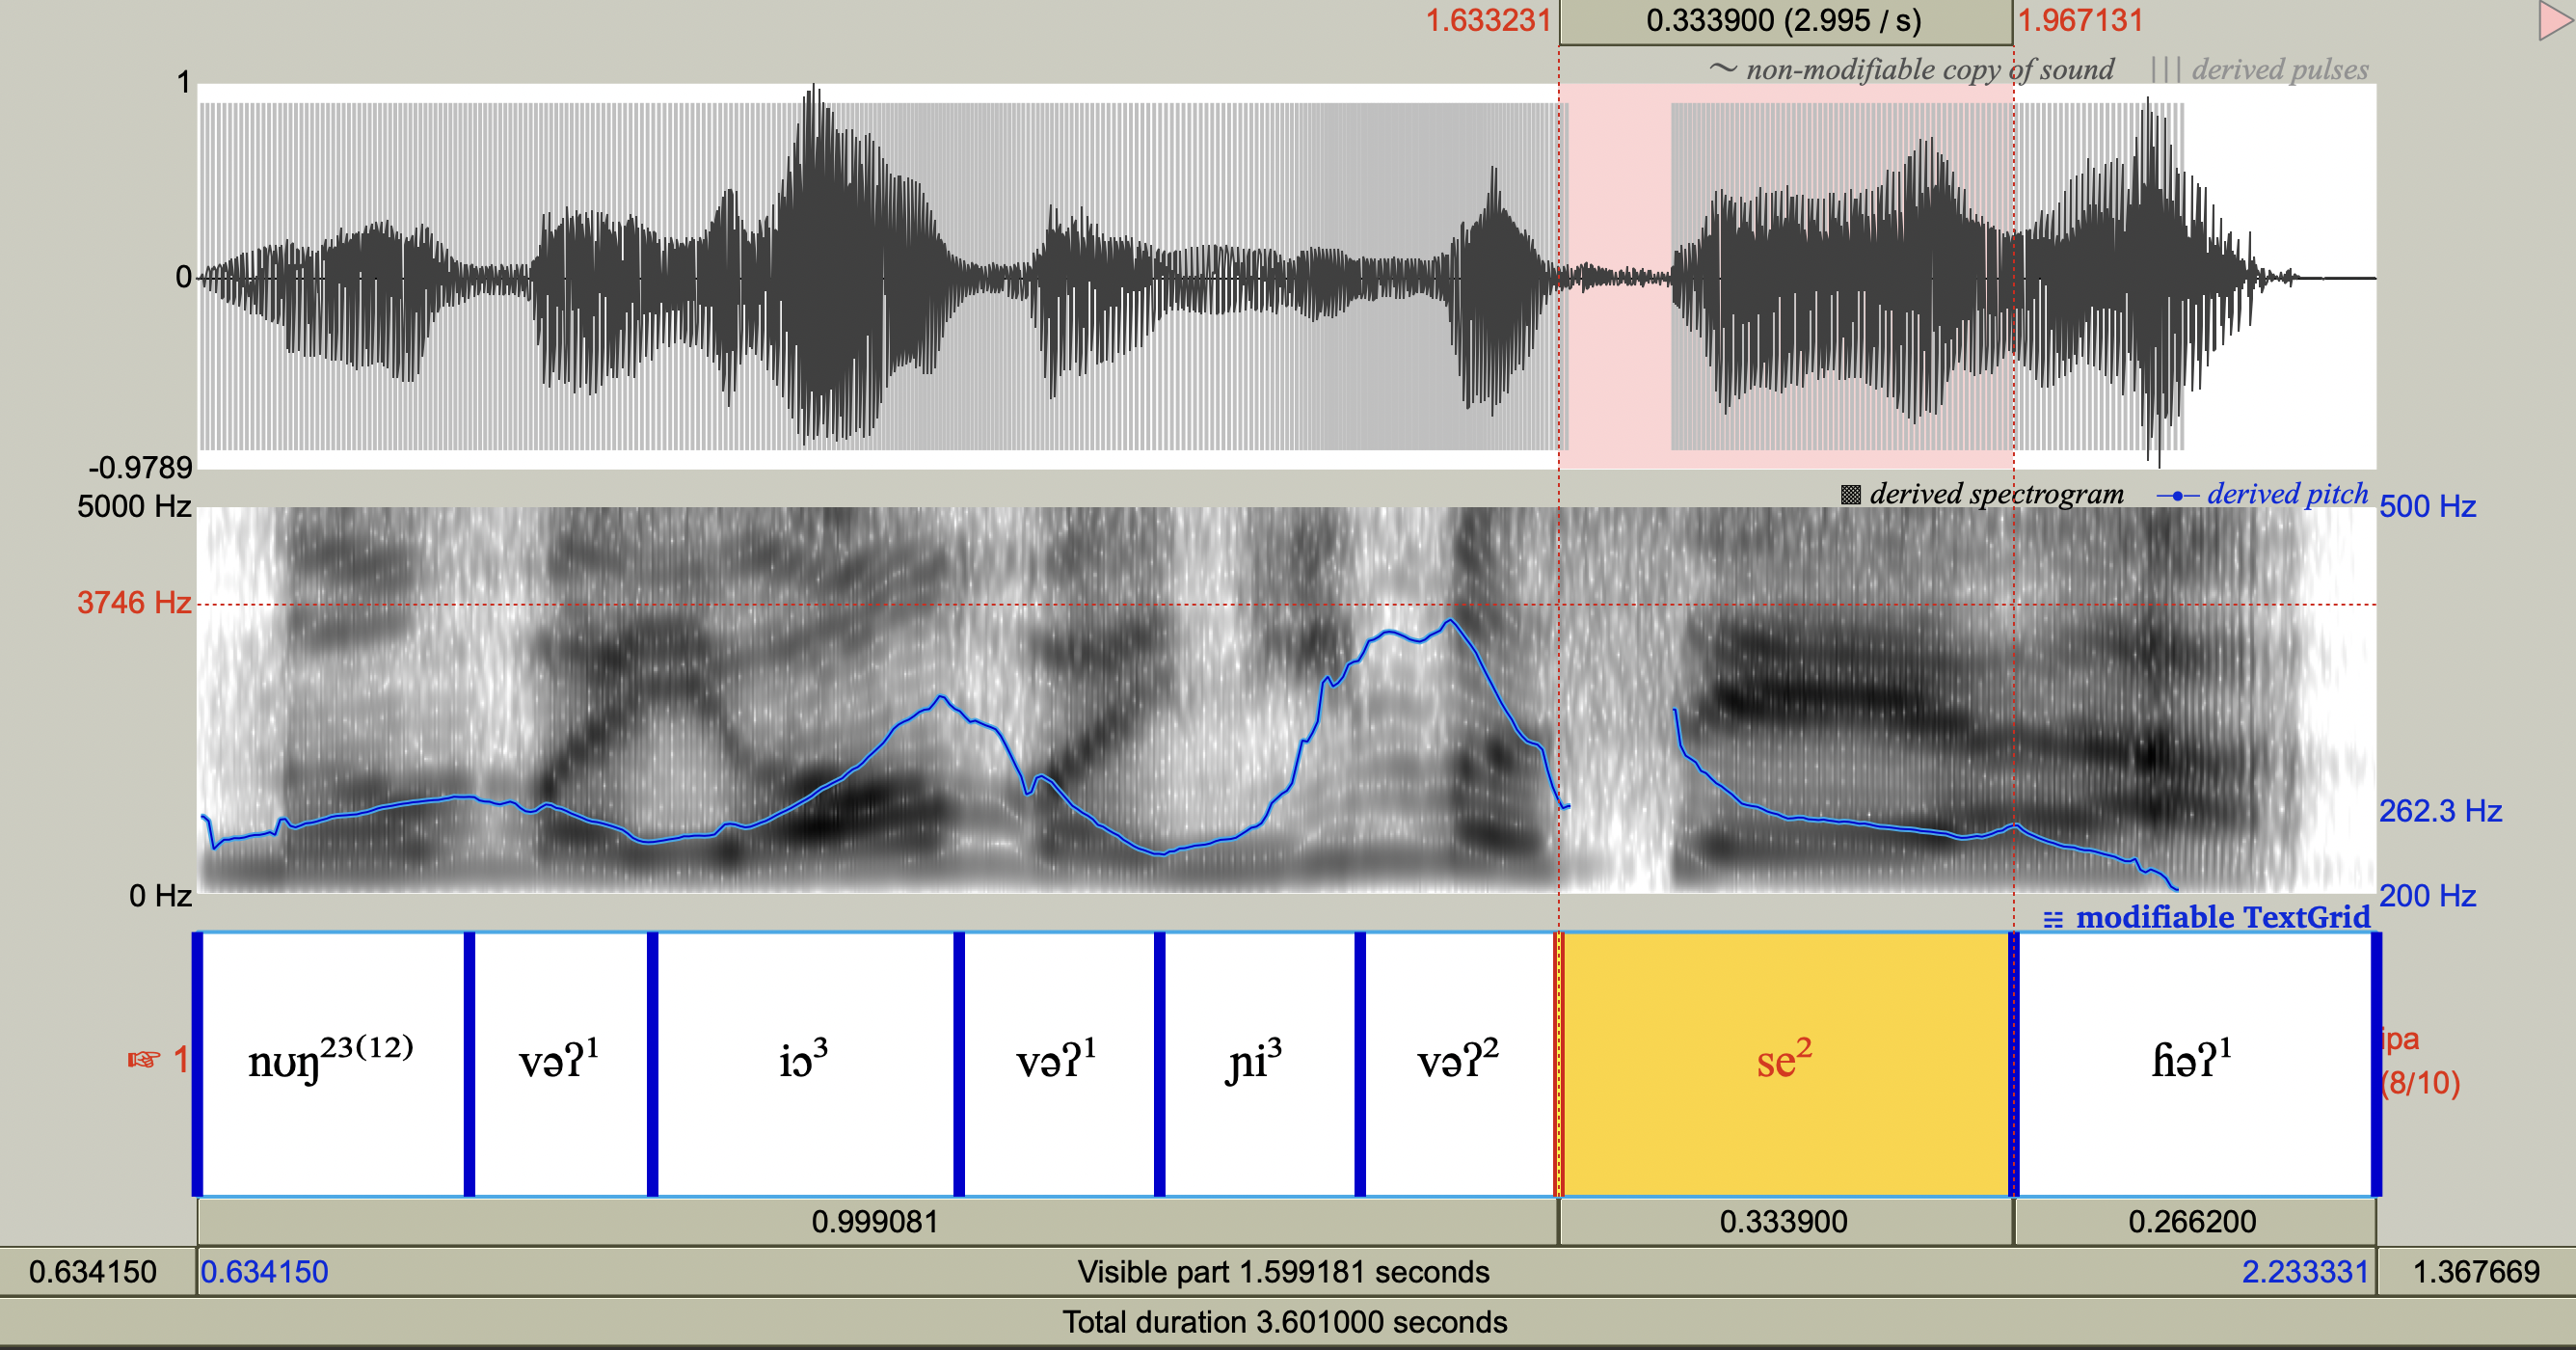
\includegraphics[width=0.6\paperwidth]{s5_sp1.png}
    \caption{Sentence 5 by speaker 1.\label{fig:s5_sp1}}
\end{figure}

\begin{figure}[H]
    \centering
    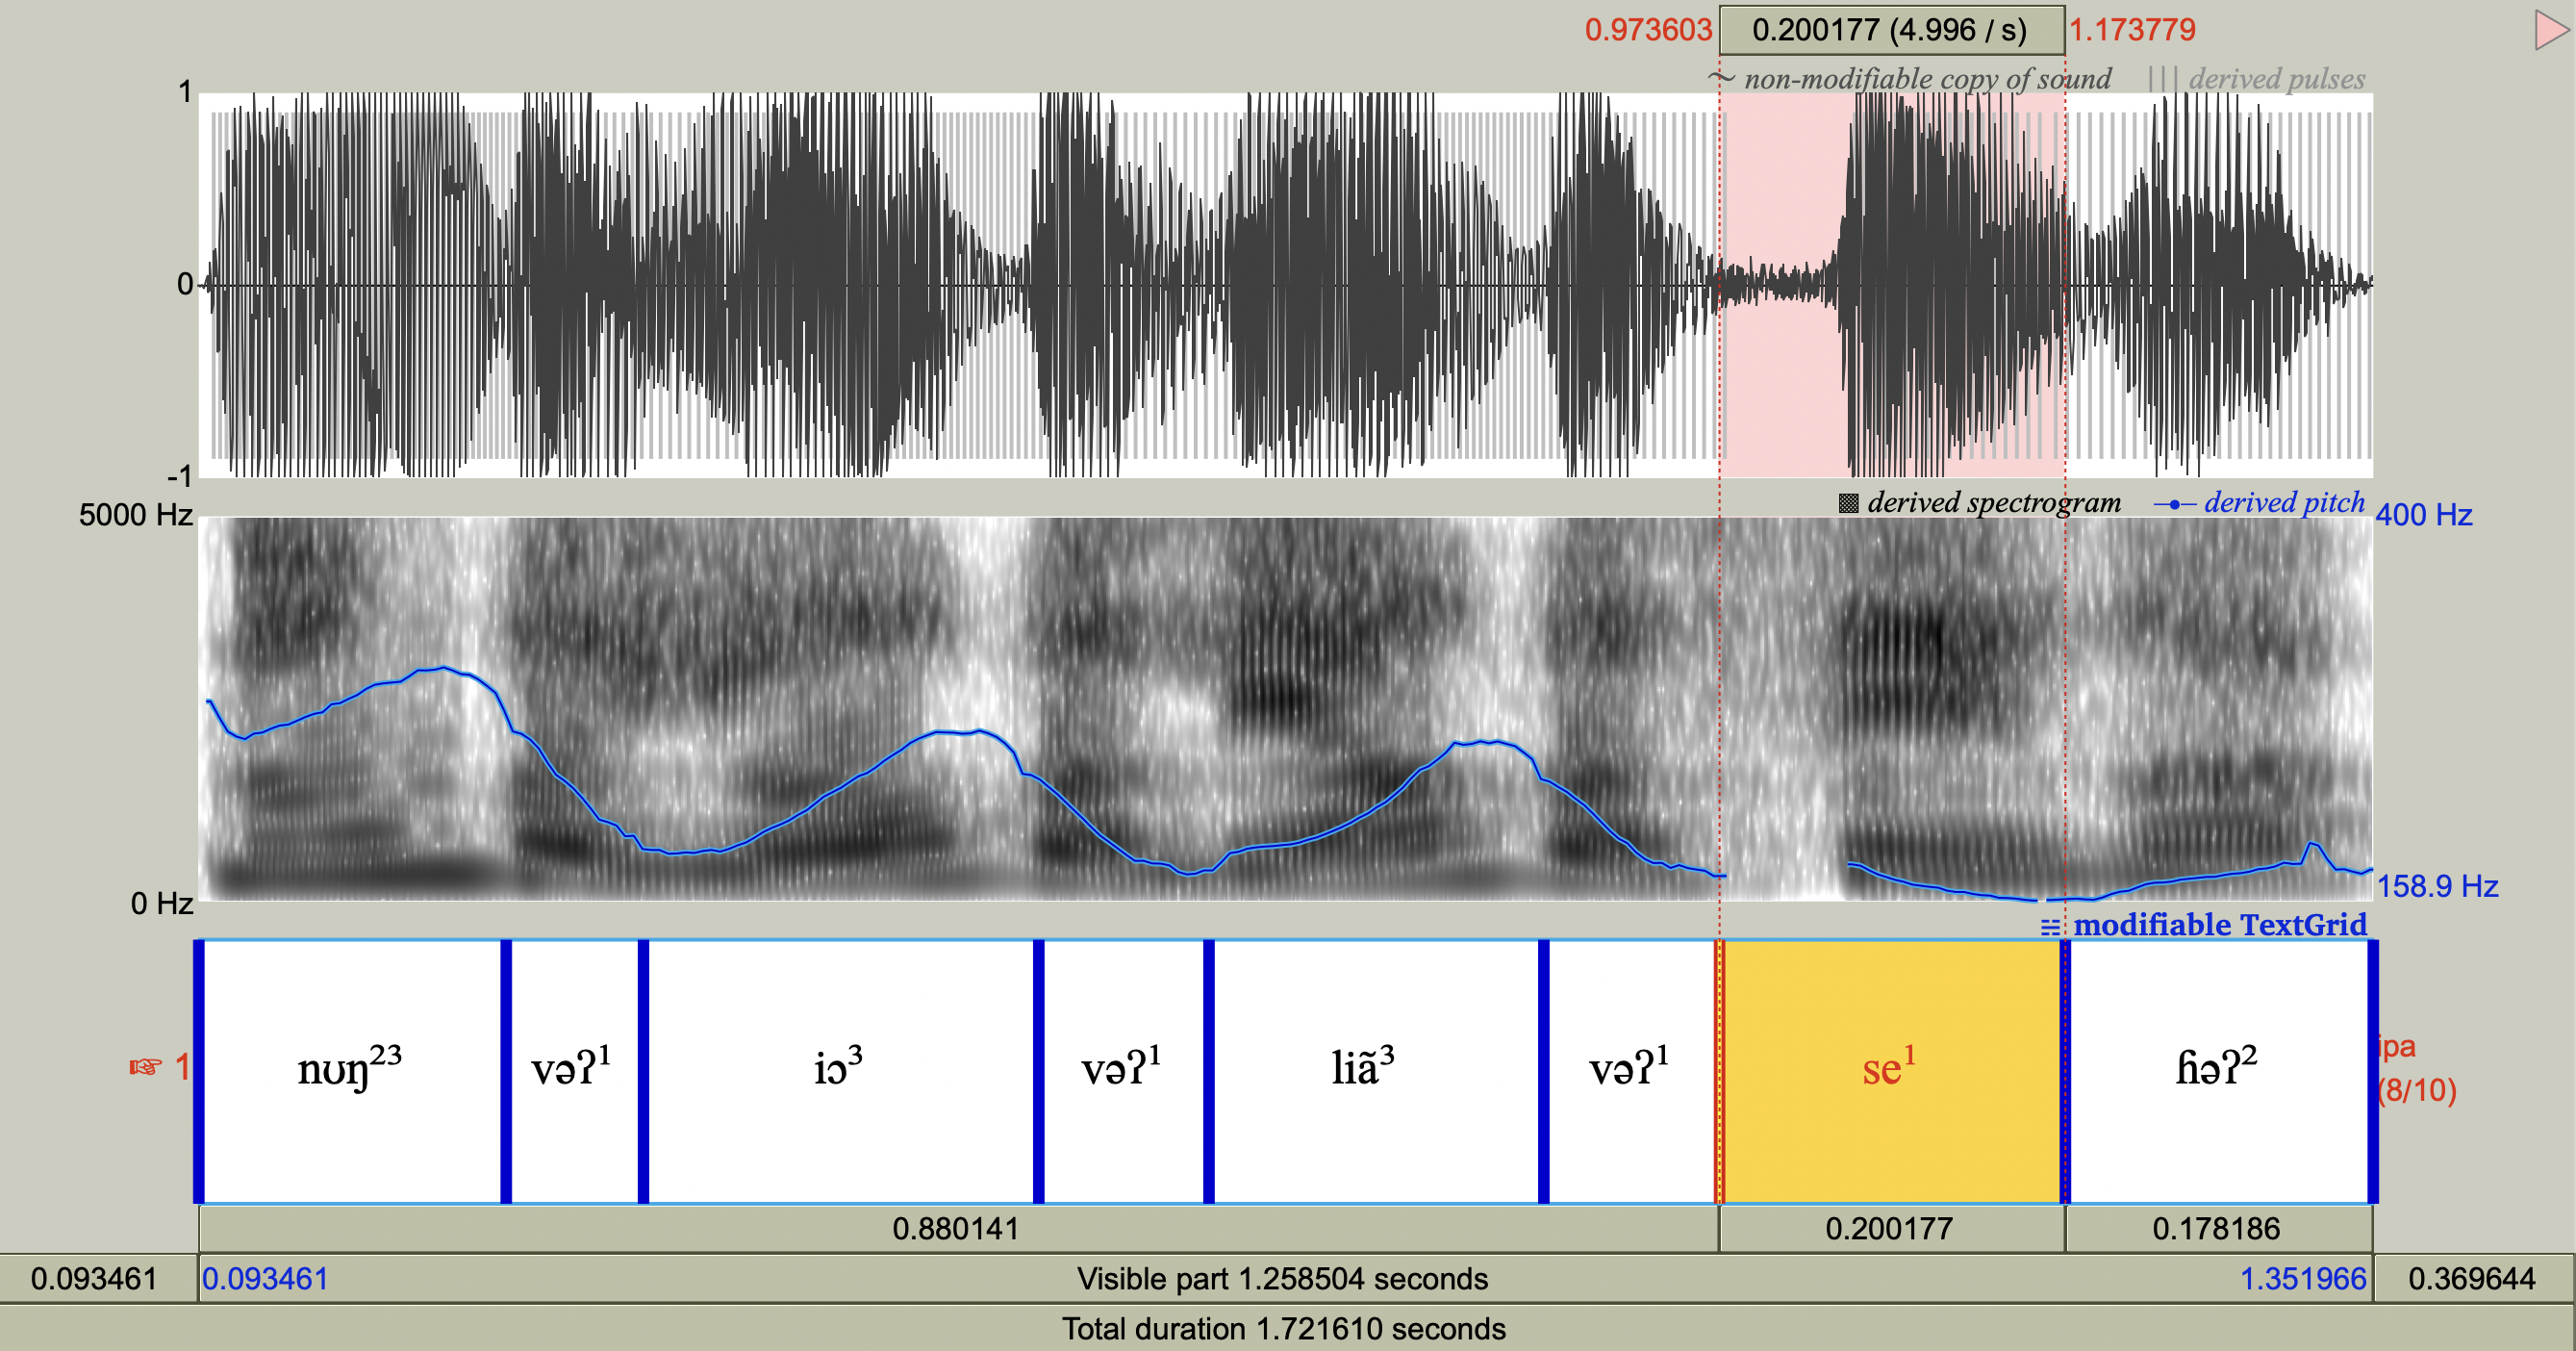
\includegraphics[width=0.6\paperwidth]{s5_sp2.png}
    \caption{Sentence 5 by speaker 2.\label{fig:s5_sp2}}
\end{figure}

\begin{figure}[H]
    \centering
    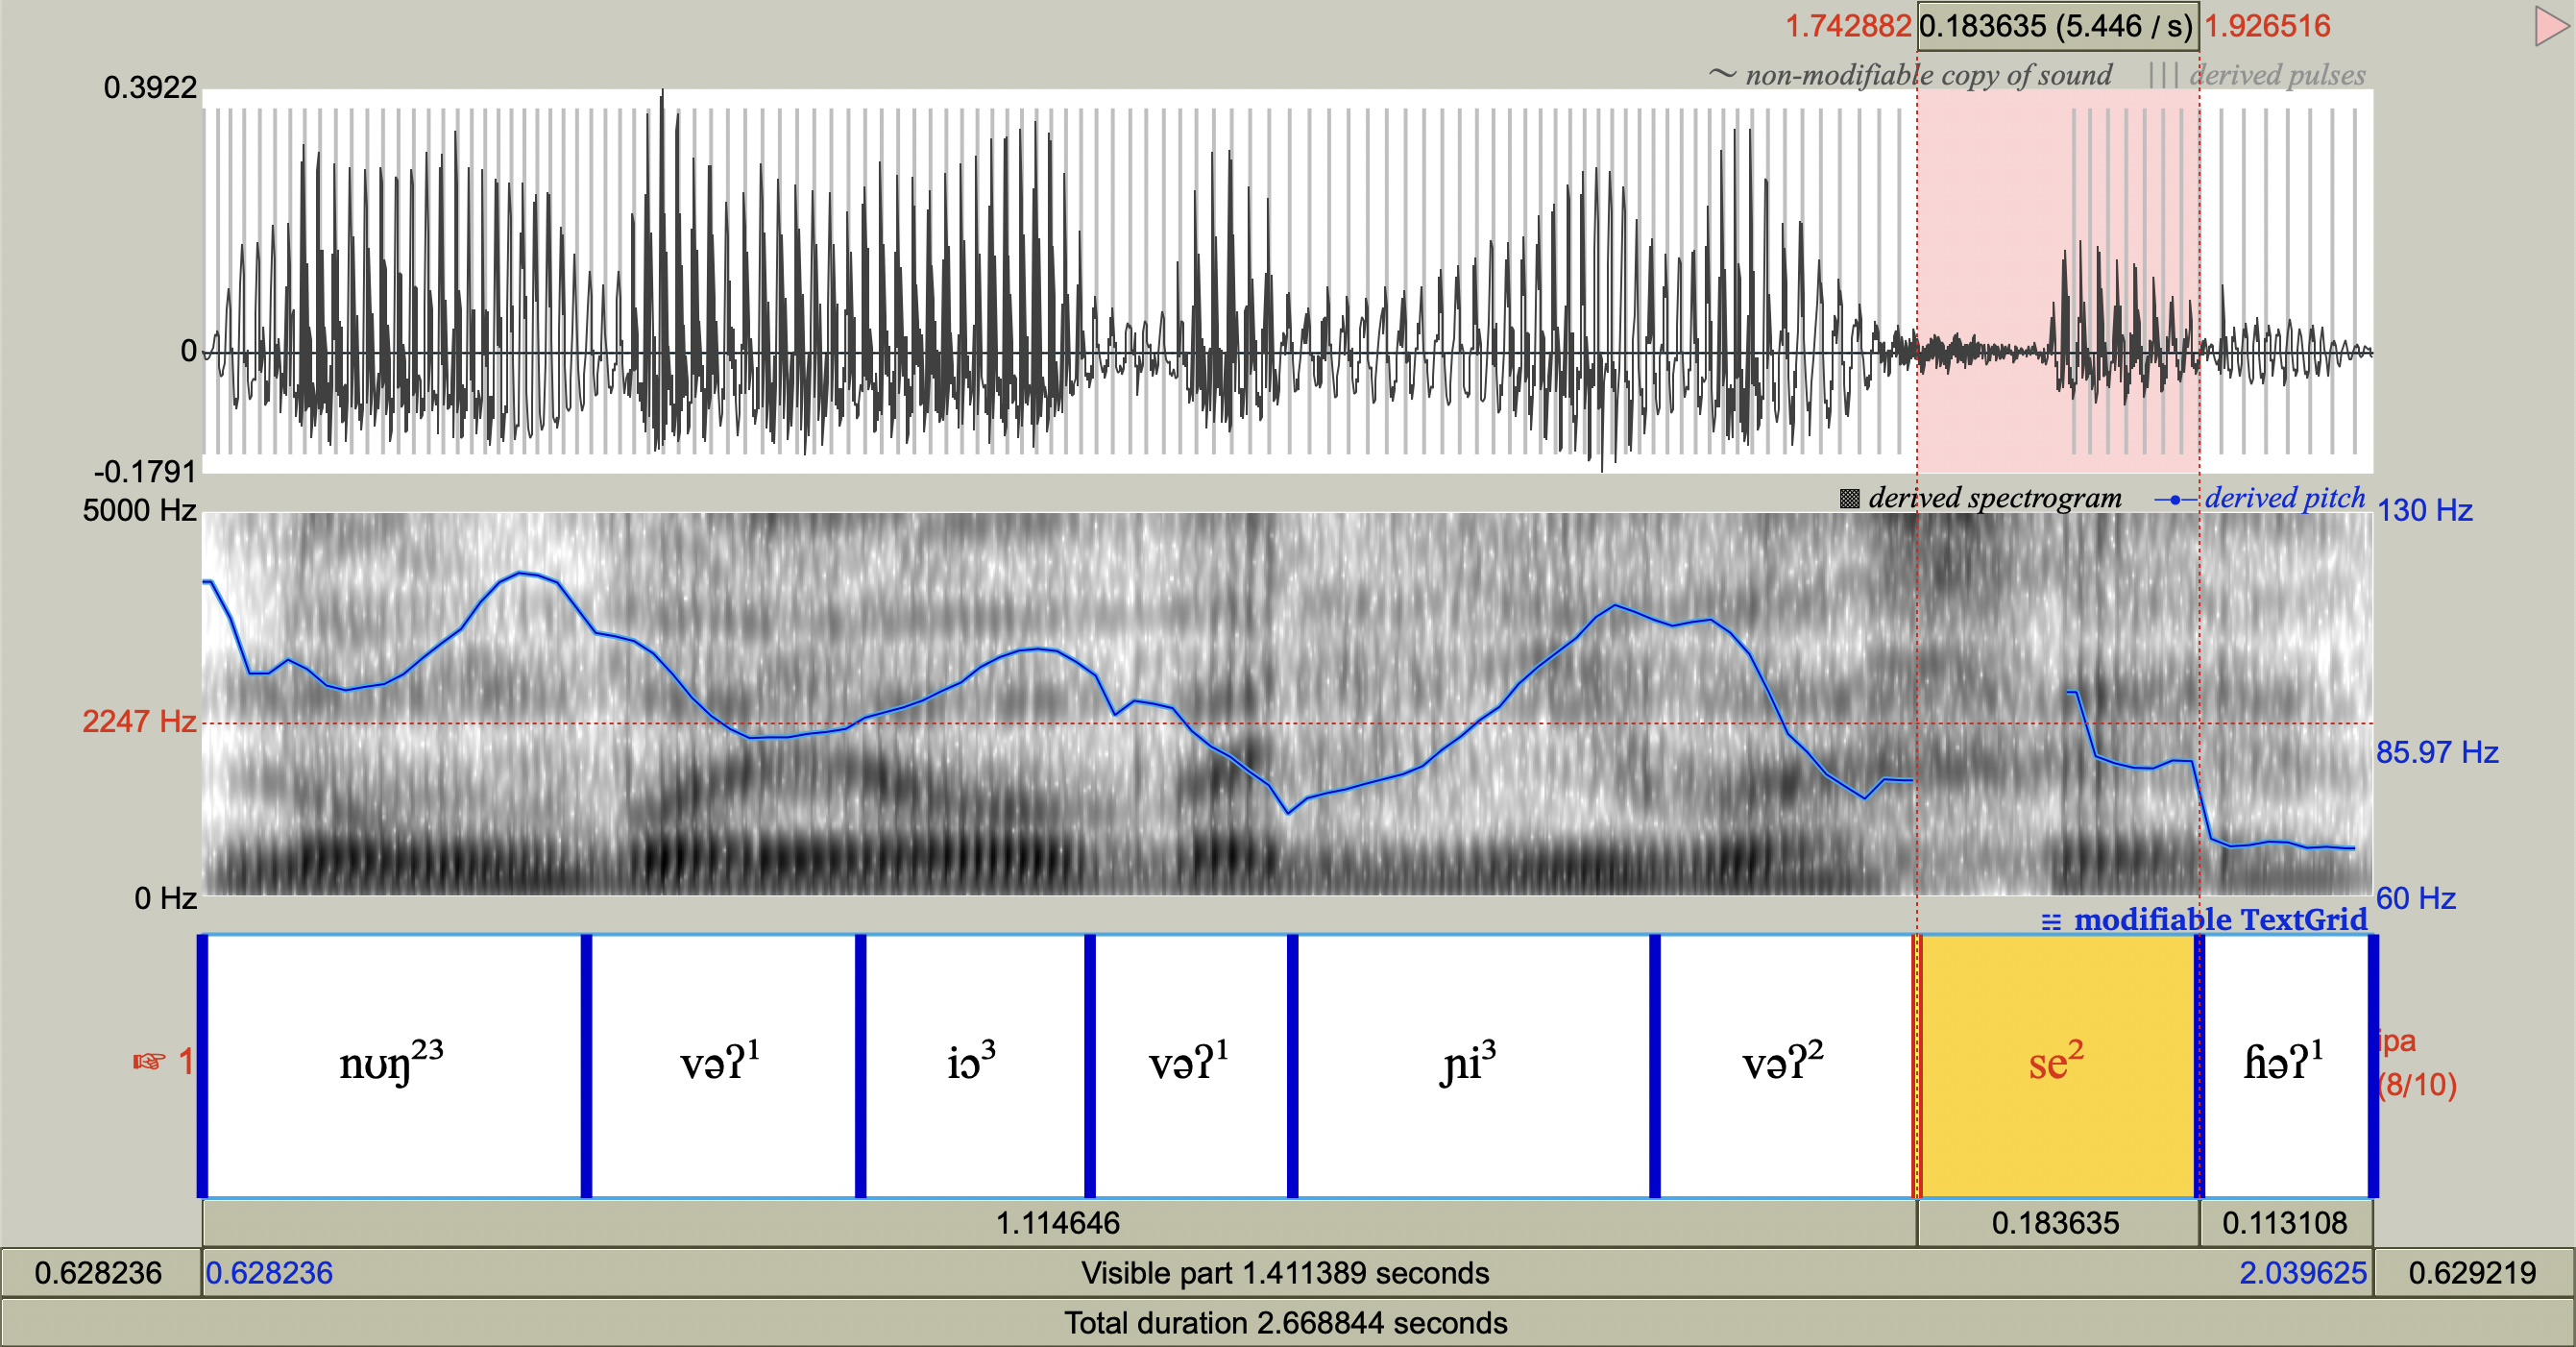
\includegraphics[width=0.6\paperwidth]{s5_sp3.png}
    \caption{Sentence 5 by speaker 3.\label{fig:s5_sp3}}
\end{figure}

\section{Questionnaire}
\begin{figure}[H]
    \centering
    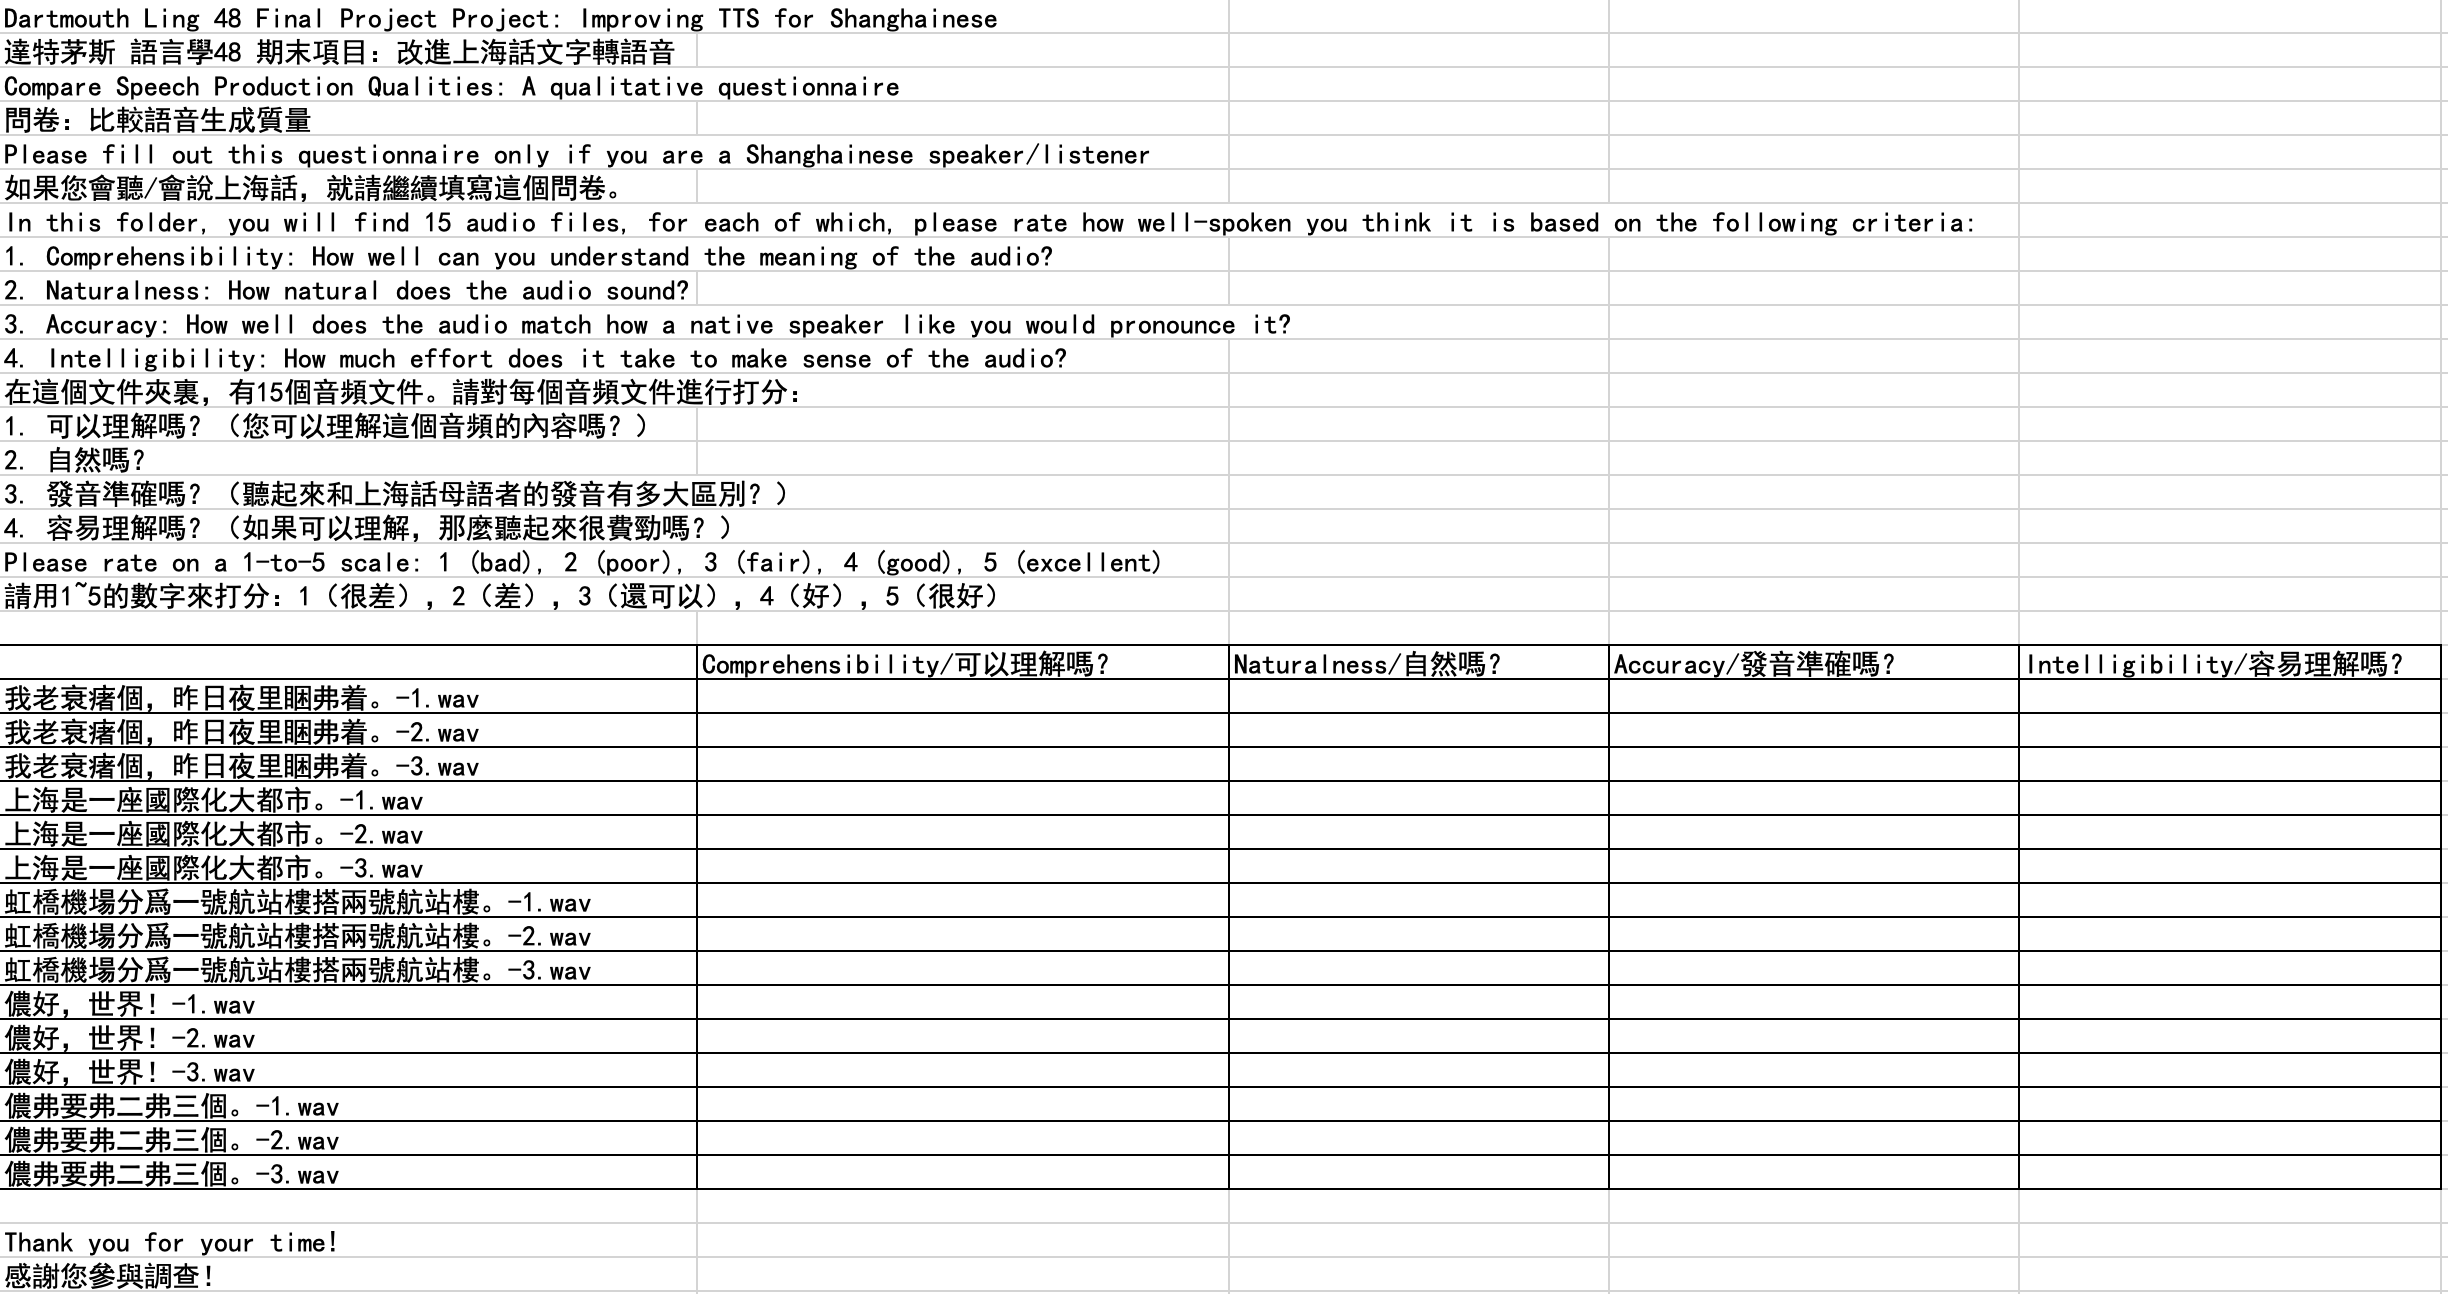
\includegraphics[width=0.6\paperwidth]{questionnaire.png}
    \caption{Questionnaire.\label{fig:questionnaire}}
\end{figure}

\end{document}
